\documentclass[spanish,11pt,letterpaper,oneside]{memoir}

% Configuración del idioma español
\usepackage[T1]{fontenc}
\usepackage[utf8]{inputenc}
\usepackage[spanish]{babel}
\usepackage{graphicx}
\usepackage{wrapfig}
\usepackage{csquotes}
% Configuración de las citas bibliográficas (puedes cambiarlo según tu preferencia)
%\usepackage[backend=biber,style=ieee]{biblatex}


% Personalización de los nombres de los capítulos y otros elementos
\renewcommand{\partname}{Parte}
\renewcommand{\chaptername}{Capítulo}
\renewcommand{\bibname}{Bibliografía}
\renewcommand{\contentsname}{Tabla de contenidos}
\renewcommand{\listfigurename}{Lista de figuras}
\renewcommand{\listtablename}{Lista de tablas}

\begin{document}
\frontmatter
% Portada
\begin{titlingpage}
  \begin{center}
  	{
\includegraphics[width=0.35\linewidth]{Sem_1/figuras/ulaLogo}\par}
  	\vspace{1cm}
	\begin{Large}
		Universidad de los Andes \\
		Facultad de Ciencias \\ 
		Departamento de Física \\ 
		Laboratorio de Física Aplicada\par
	\end{Large}
	\vspace{0.7cm}
	\textbf{{\Large Búsqueda de agrupaciones en data proveniente de electrocardiogramas (ECG), mediante el Análisis de Componentes Principales (PCA) y el uso de Redes Neuronales.}}\par
	\vspace{0.5cm}
	{\itshape\large Trabajo especial de grado.}\par
	\vspace{0.5cm}
	{\large\textbf{Br. Abrahan David Quintero Teran}}\par
   	\vspace{0.5cm}
    {\large Tutor: Prof. Juan Villegas}\par
    \vspace{0.5cm}
    \begin{flushright}
    	{\large Jurados: \par
    	Prof. Marcos Rodríguez \par
    	Prof. John Ferreira \par}
    \end{flushright}
    {\large\textbf{Mérida -- Venezuela}} \par
    {\large 2024} % Deja esto vacío para eliminar la fecha de la portada
  \end{center}
\end{titlingpage}

% Abstract en español
\begin{abstract}
  Este es el resumen de mi tesis.
\end{abstract}
\newpage
% Abstract en inglés (opcional)
% \begin{otherlanguage}{english}
% \begin{abstract}
% This is the abstract of your thesis in English.
% \end{abstract}
% \end{otherlanguage}

\tableofcontents*
\mainmatter


%\part{Primer Seminario}
\pagestyle{empty}{\huge\textbf{Introducción}}
\chapter{El problema}
	El electrocardiograma (ECG) es una técnica no invasiva que permite registrar y medir las señales eléctricas generadas por el corazón. Consiste en la captación de la variación temporal del potencial bioeléctrico durante cada ciclo cardíaco, utilizando electrodos colocados en la superficie cutánea del paciente \cite{ZHANG2021113}. El análisis del ECG proporciona datos sobre el sistema cardiovascular, en particular el corazón, lo que permite detectar diversas enfermedades que pueden afectar su funcionamiento óptimo. Estas enfermedades incluyen arritmias cardíacas, obstrucción de arterias, insuficiencia cardíaca y ataques al corazón \cite{MedlineECG}.\\ Según la organización mundial de la salud \cite{Who}, las enfermedades cardiovasculares (ECV) son las principal causa de muerte en hombres y mujeres en el mundo, con alrededor de 17,9 millones de personas que mueren al año a causa de estas. Entre los numerosos factores que llevan a esta consecuencia, se encuentran los errores provenientes de la interpretación manual de los electrocardiogramas (ECGs), por lo general, los médicos emplean características heurísticas diseñadas manualmente o utilizan arquitecturas de aprendizaje de características superficiales, esto puede generar como consecuencia, variabilidad entre los diagnósticos de los observadores e identificación de anomalías incorrectas que pueden llevar a ocasionar diagnósticos imprecisos y en consecuencia, tratamientos inadecuados. Además estos métodos manuales que utilizan arquitecturas de aprendizaje de características superficiales descartan información relevante del ECG inmersa dentro de características que no son superficiales, lo que provee una baja exactitud en el diagnostico a partir de las señales por lo que siempre será necesario de la supervisión de un experto con el fin de corregir estos errores. 

\section{Justificación}
	Ante la necesidad de reducir los errores provenientes de la interpretación manual de los ECGs que junto con la presencia de ruidos e interferencias en las señales complican aún más el análisis del ECG surge la necesidad de desarrollar herramientas que ayuden a reducir estos errores. Por lo que la identificación de patrones específicos y la clasificación precisa en grupos de pacientes siguen siendo desafíos importantes, ya que los métodos tradicionales de análisis de ECGs a menudo no son lo suficientemente robustos para manejar estas complejidades de manera eficiente. Es por esto que el desarrollo de herramientas que favorezcan la debida identificación de diversas enfermedades cardiovasculares, puede tener un impacto positivo en el proceso de diagnostico de enfermedades y facilitar tratamientos oportunos.
	
\section{Antecedentes}
    Desde finales del siglo pasado ha habido un creciente interés en los métodos computacionales aplicados a la salud, por ejemplo en 1985, Pan y Tompkins \cite{PanTompkins85} diseñaron un algoritmo para detección de los complejos QRS en tiempo real y con bajo costo computacional, este algoritmo sentó las bases de la implementación de algoritmos de detección y análisis para las señales de electrocardiogramas. En 1996, Laguna \textit{et al.} \cite{Laguna97} presentaron un sistema de estimación del modelo de Hermite adaptativo (AHMES) para la estimación en línea latido a latido de las características que describen el complejo QRS con el modelo de Hermite. Gómez Herrero \textit{et al.} \cite{Herrero05}, presentaron un algoritmo conocido como ``Matching Pursuit'' que ofrece la capacidad de descomponer cualquier señal en un combinación lineal de formas de onda extraídas de un diccionario redundante de funciones llamado Gabor. Este algoritmo se ha reconocido como una herramienta eficaz para realizar transformaciones adaptativas de tiempo-frecuencia en señales de ECG, lo que permite obtener características relevantes en el dominio tiempo-frecuencia. \\
    \\
    Siguiendo esta linea de algoritmos que realizan transformaciones adaptativas en el dominio tiempo-frecuencia, se encuentran Martínez \textit{et al.} \cite{Martinez04} quienes proponen un delineador de ECG basado en las transformadas Wavelet (TW), para así poder detectar los inicios, picos y finales de las ondas P y T como también las ondas individuales del complejo QRS incluyendo el inicio y fin del complejo, todo esto para luego determinar los diversos intervalos y segmentos dentro del ECG, este método propuesto es tan robusto que no se ve afectado por los diversos ruidos que pueden existir dentro del ECG como lo es por ejemplo, el desplazamiento de la linea base. Para remover este ultimo, Sharma y Sharma en 2015 \cite{Sharma15} usan la Descomposición Vibracional de Hilbert (HVD) para descomponer la señal original del ECG en una serie de funciones modales intrínsecas y luego remover el primer termino, que corresponde a la componente de mayor energía y así eliminar el desplazamiento de la linea base del ECG. \\
    \\
    Otros métodos relevantes usando para la extracción de características a partir de dominios transformados, tales como la Transformada de Coseno Discreta (DCT), la Transformada Wavelet Continua (CWT) y la Transformada Wavelet Discreta (DWT), estas técnicas permiten analizar las señales de ECG en diferentes representaciones y obtener características significativas para su posterior procesamiento y análisis, así Khorrami y Moavenian en 2010 \cite{Khorrami10} utilizaron las CWT, DWT y DCT, con el fin de mejorar la capacidad de dos clasificadores de patrones en la clasificación de arritmias ECG. \\
    \\
    Song \textit{et al.} (2005) \cite{Song05} extrajeron diecisiete características de entrada originales de señales pre-procesadas mediante TW, utilizando el análisis discriminaste lineal (LDA). El rendimiento del clasificador SVM (Máquina de Soporte Vectorial) con características reducidas por LDA mostró ser mayor que con el Análisis de Componentes Principales (PCA) e incluso con características originales, sin embargo, está técnica requirió de un mayor costo computacional. Yu y Chen (2007) \cite{Yu07} utilizaron la transformación wavelet y una red neuronal probabilística (PNN), para descomponer las señales de latido de ECG en diferentes sub-bandas utilizando la DWT. Posteriormente, seleccionaron tres conjuntos de características estadísticas de las señales compuestas para caracterizar las señales de ECG, así como la potencia de AC y el intervalo RR instantáneo de la señal original.\\
\\
    Ye, Coimbra y Kumar (2010) \cite{Ye10} propusieron un enfoque de combinación de características morfológicas y dinámicas refiriéndose a la TW y el análisis de componentes independientes (ICA) aplicándose por separado a cada latido del corazón para extraer los coeficientes correspondientes como características morfológicas. Además concatenaron la información del intervalo RR y estos dos tipos diferentes de características y se utilizó SVM para la clasificación. Rojas, Medina y Dugarte (2011) \cite{Dugarte11} diseñan un sistema multicanal de adquisición y analizan la señal electrocardiográfica de alta resolución, en el que utilizan Máquinas de Soporte Vectorial de mínimos cuadrados (LSSVM) para determinar el inicio del complejo QRS y el final de la onda T, entrenadas en base a atributos extraídos de la señal preprocesada y de señales obtenidas mediante descomposiciones con Wavelets. Estas técnicas permiten estimar el intervalo QT así como el intervalo QT corregido (QTc).\\
    \\
    También Zhang \textit{et al.} (2024) \cite{Zhang24} proponen un modelo de Redes Neuronales Convolucionales (CNN) para clasificar insuficiencias cardíacas por clases, según la Asociación del Corazón de Nueva York, a partir de imágenes electrocardiográficas en el que consiguen el mejor resultado segmentando las imágenes en fragmentos de 12 segundos. Así también Astudillo \textit{et al.} (2024) \cite{Astudillo24} prueban cinco arquitecturas de CNN diferentes para clasificación de arritmias cardíacas. Estas dos ultimas investigaciones consiguen predicciones superiores al 98.98\% en el mejor de los escenarios. \\
    \\
    En este sentido, Pan y Tompkins obtuvieron un 99.3\% de complejos QRS detectados haciendo uso de la base de datos MIT-BIH Arritmia (MITDB) \cite{PanTompkins85}. El sistema que Laguna \textit{et al.} \cite{Laguna97} presentan, mejora la relación señal-ruido (SNR) en la estimación, lo que permite la adaptación a los cambios del QRS latido a latido, proporcionando una descripción de la evolución de la señal QRS y la compresión de datos del ECG. El sistema AHMES permite la estimación en línea de estas características con una mejor SNR que la estimación directa. Martínez \textit{et al.} \cite{Martinez04} usando MITDB encuentran un 99.8\% de complejos QRS detectados, un resultado superior al obtenido por Pan y Tompkins. Gómez Herrero \textit{et al.} \cite{Herrero05} usando la base de datos MITDB e introduciendo Análisis de Componentes Independientes (ICA) como extractor de características para el procesamiento del ECG para la simulación, obtienen resultados con una precisión de 99.8\% para clasificar latidos que corresponden a la clase de Ritmo Sinusal Normal (RSN) y 97.9\% para latidos de la clase de Contracción Ventricular Prematura (PVC). Así también Sharma y Sharma \cite{Sharma15} compara su método usando criterios de correlación y SNR donde concluyen que la técnica propuesta se desempeña mejor en la mayoría de los casos que técnicas anteriores para remover el desplazamiento de la linea base. Song \textit{et al.} \cite{Song05} identificaron seis tipos diferentes de arritmias obteniendo una exactitud del 98.94\%. Ye, Coimbra y Kumar \cite{Ye10} reconocieron 15 clases de latidos con una exactitud del 99.66\% en un grupo de prueba de 85945 muestras. Khorrami y Moavenian \cite{Khorrami10}, utilizando SVM y la base de datos MITDB con dos conjuntos de datos de prueba con diferentes configuraciones obtuvieron un error cuadrático medio (MSE) de 0.14 y 0.15 respectivamente para cada prueba.\\
    \\
    Rojas, Medina y Dugarte \cite{Dugarte11} encuentran diferencias estadísticas significativas importantes entre pacientes chagásicos y pacientes de control de esta manera logran abordar la detección temprana y no invasiva de enfermedades cardiovasculares como el mal de Chagas.   \\
 

\section{Objetivos}
\subsection{Objetivo General}
Analizar los datos provenientes de electrocardiogramas mediante la aplicación de análisis de componentes principales (PCA) y redes neuronales, con el objetivo de identificar agrupaciones en dicha data.
\subsection{Objetivos específicos}
\begin{enumerate}
	\item Analizar y catalogar los datos de los electrocardiogramas para mejorar la calidad de los datos y la precisión de los modelos predictivos.
	\item Desarrollar un marco metodológico solido que combine el análisis de componentes principales (PCA) y redes neuronales para la identificación de grupos de datos.
	\item Evaluar el rendimiento de los modelos propuestos utilizando los datasets de Physionet.
\end{enumerate}



\chapter{Marco Teórico}

\section{Conceptos básicos}
\subsection{Introducción al Electrocardiograma (ECG)}
	La humanidad siempre, en su continuo deseo de aprender y entender más, ha querido desentrañar los secretos del cuerpo humano entendiendo su funcionamiento interno. Al principio con técnicas invasivas acordes a la tecnología disponible a la época, pero evolucionando continuamente, creando así exámenes cada vez menos invasivos, con el fin de mejorar el diagnostico, siendo mas preciso y oportuno. Entre esos exámenes se destaca el electrocardiograma (ECG) el cual es una representación visual de la actividad eléctrica del corazón en función del tiempo, que se obtiene desde la superficie corporal, con un electrocardiógrafo, este es el instrumento principal de la electrofisiología cardíaca y tiene una función relevante en el cribado y diagnóstico de las enfermedades cardiovasculares, alteraciones metabólicas y demás utilidades. \\
	\\

    El primer «electrograma» humano fue publicado en 1887 por el fisiólogo británico Augustus Desiré Waller, de la St. Mary's Medical School de Londres. Utilizó un electrómetro capilar de Lipmann con electrodos aplicados a la espalda y el tórax del sujeto. Demostró que la contracción ventricular precedía a la actividad eléctrica. En su primer informe sobre un registro de la electricidad cardíaca realizado en la superficie corporal, Waller utilizó el término «cardiógrafo».  \\
    \\
    Einthoven empezó a experimentar con el potencial del capilar para captar corrientes eléctricas diminutas. En 1895 demostró cinco deflexiones que denominó ABCDE en 1895. Creó un ajuste matemático para para tener en cuenta la inercia del sistema capilar, lo que produjo las curvas de corriente que vemos hoy en día. Siguiendo la tradición matemática establecida por Descartes, utilizó la parte terminal de la serie parte terminal de la serie alfabética (PQRST) para denominar estas derivaciones. \\
    \\
    El pionero de la electrocardiografía, Waller dijo a finales de 1911: «No creo que la electrocardiografía vaya a tener un uso extensivo en los hospitales. A lo sumo puede tener un uso raro y ocasional para proporcionar un registro de alguna anomalía de la actividad cardíaca». Sin embargo, diez años de los estudios clínicos de Einthoven con los galvanómetros de cuerda transformaron este curioso fenómeno fisiológico en un dispositivo de registro clínico indispensable. Las asociaciones de la inversión de la onda T con la angina de pecho y la arteriosclerosis. en 1910, junto con otras arritmias, como el bigeminismo, bloqueo cardíaco completo, hipertrofia ventricular derecha e izquierda, fibrilación y aleteo auricular y ejemplos de diversas cardiopatías. Con su nueva técnica, estandarizó los trazados y formuló el concepto de «triángulo de Einthoven» relacionando relacionando matemáticamente las 3 derivaciones (Derivación III = Derivación II - Derivación I). En 1924, el «Padre de la electrocardiografía» recibió el Premio Nobel de Medicina \cite{vincent2022}.\\
    \\
    En 1957, el médico estadounidense Norman Jefferis Holter inventó el ECG dinámico (DCG), a menudo conocido como Holter, en uno de los primeros intentos de combinar monitorización clínica y movilidad. Creó una mochila que pesaba unos 38 kg y tenía un dispositivo que podía registrar la actividad cardíaca del participante. Este portátil permite la monitorización continua de actividad eléctrica del sistema cardiovascular durante 24 horas, lo que ayuda a estudiar las arritmias y a localizar el lugar de la isquemia miocárdica. Reconociendo los beneficios potenciales de un dispositivo de monitorización de este tipo, Holter consiguió convertir su idea en una valiosa herramienta de diagnóstico reduciendo el tamaño y el peso a 1 kg con ayuda de Del Mar Avionics, un conocido fabricante de equipos aeronáuticos \cite{vincent2022}.\\
    \\
    Durante las tres primeras décadas del siglo 20, el ECG de tres derivaciones periféricas fue largamente usado, especialmente luego de mejoras que lo hicieron más portable. A pesar de que el ECG de tres derivaciones era una manera fiable de evaluar arritmias, pronto se reconoció que el corazón incluía «zonas silenciosas» en las que un infarto de miocardio podría no ser detectado. En 1942, Emanuel Goldberger construyó las derivaciones precordiales (unipolares) usando el promedio de las diferencias de potencial de las tres derivaciones periféricas como terminal de referencia, que inicialmente fue creado por Frank N. Wilson, al cual se le conoce como terminal central de Wilson, que ahora se denominan como derivaciones precordiales (V1-V6), donde en 1938, la Asociación Americana del Corazón (AHA) y la Sociedad Cardiaca de Gran Bretaña recomendaron la estandarización del posicionamiento de los electrodos en el pecho para dichas derivaciones. También Goldberger propuso una manera de obtener lo que ahora se llaman derivaciones aumentadas, conocidas por las siglas a-VL, a-VR, y a-VF. 8 años después la AHA recomendó la estandarización del ECG de 12 derivaciones. \cite{vincent2022}\\
    \\
    En la era digital, la tecnología del silicio y los circuitos circuitos impresos han hecho posible la miniaturización electrónicos. Desde hace algún tiempo, la tecnología ha ganado popularidad en el campo de la medicina y la necesidad de los clientes de controlar su salud ha sido el principal motor. La influencia de los "vestibles" (wearables) ha hecho inevitable la continua investigación y desarrollo de nuevas funciones que pueden evaluar y transmitir datos biométricos en tiempo real. \\

    
    
    
    
    
	El corazón consta de cuatro partes, dos aurículas y dos ventrículos, el ECG registra los impulsos eléctricos que estimulan estas partes y producen su contracción. Las células cardíacas en reposo se encuentras cargadas o polarizadas; pero la estimulación eléctrica las "despolariza", y se contraen. \\
	\begin{figure}[h]
		\centering
		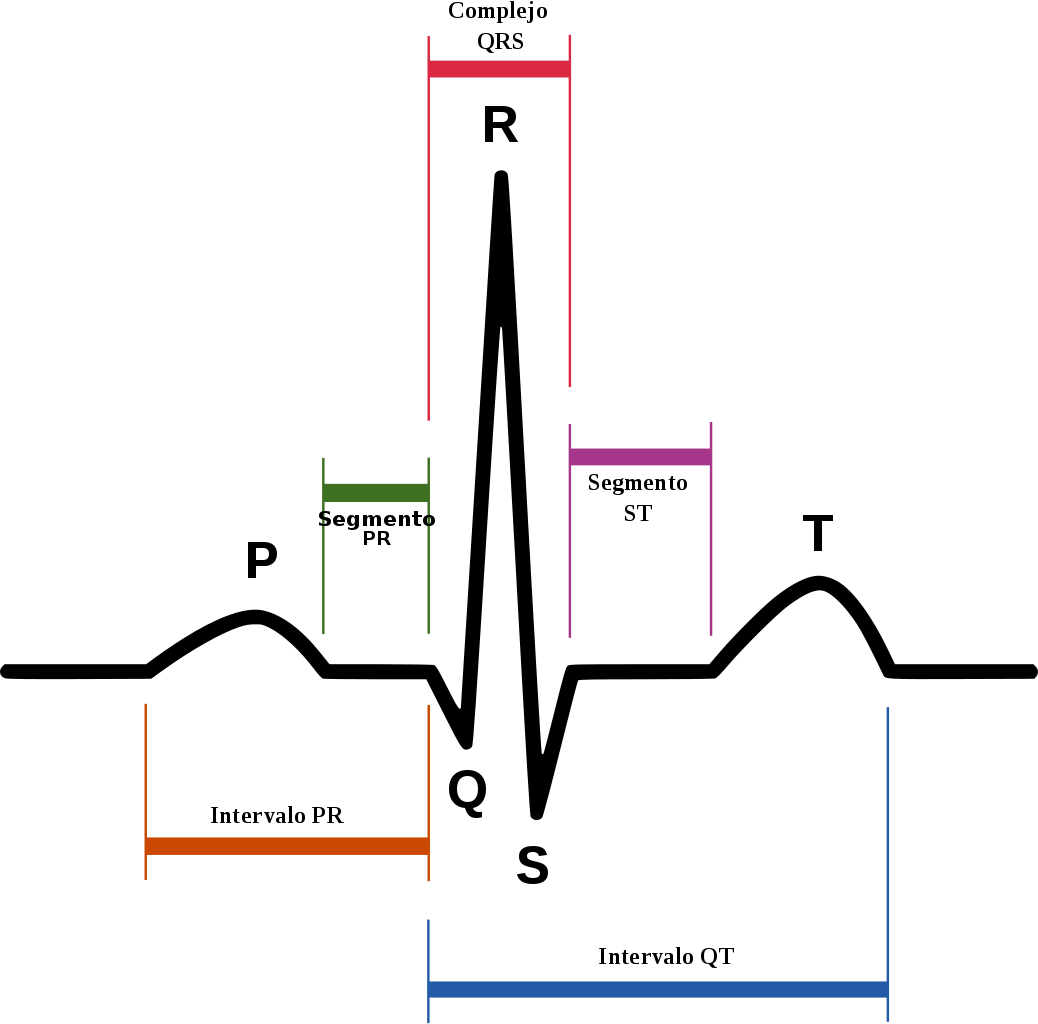
\includegraphics[width=0.5\linewidth]{Sem_1/figuras/1038px-SinusRhythmLabels-es.svg}
		\caption{ECG del corazón con ritmo sinusal normal}
		\label{fig:ECGSinusal}
	\end{figure}
	\\
	Como se observa en la figura \ref{fig:ECGSinusal} el ECG consta de varias ondas representativas de cada etapa de un latido cardíaco, estas son: \\
	\begin{itemize}
		\item \textbf{Onda P}: registra la despolarización auricular.
		\item \textbf{Complejo QRS}: Es la despolarización ventricular.
		\item \textbf{Onda T}: representa la repolarización ventricular.
	\end{itemize}

\section{Conceptos específicos}
\subsection{Análisis de Componentes Principales (PCA).}
	Los grandes conjuntos de datos están cada vez más extendidos en muchas disciplinas. Para interpretarlos, se necesitan métodos que reduzcan drásticamente su dimensionalidad de forma interpretable, de modo que se conserve la mayor parte de la información contenida en los datos. Se han desarrollado muchas técnicas con este fin, pero el análisis de componentes principales (PCA) es una de las más antiguas y utilizadas. Su idea es sencilla: reducir la dimensionalidad de un conjunto de datos conservando la mayor cantidad posible de «variabilidad» (es decir, de información estadística).
	
	Esto significa que «preservar tanta variabilidad como sea posible» se traduce en encontrar nuevas variables que sean funciones lineales de las del conjunto de datos original, que maximicen sucesivamente la varianza y que no estén correlacionadas entre sí. Encontrar esas nuevas variables, los componentes principales (PC), se reduce a resolver un problema de auto-valores y auto-vectores. \\
	
	Hasta que no se generalizó el uso de ordenadores electrónicos, que fue posible utilizarlo con conjuntos de datos que no fueran trivialmente pequeños. Desde entonces, su uso se ha multiplicado y se han desarrollado numerosas variantes en muchas disciplinas diferentes. Desde entonces, su uso se ha multiplicado y se han desarrollado numerosas variantes en muchas disciplinas diferentes. 
	
	La definición formal de PCA, en un contexto estándar, junto con una derivación que muestra que puede obtenerse como la solución a un problema de auto-valores y auto-vectores o, alternativamente, a partir de la descomposición del valor singular (SVD) de la matriz (centrada) de datos. El PCA puede basarse en la matriz de covarianzas o en la matriz de correlaciones. Se discutirá la elección entre estos análisis. En ambos casos, las nuevas variables (las PC) dependen del conjunto de datos, en lugar de ser funciones de base predefinidas, por lo que son adaptativas en sentido amplio. Los principales usos del PCA son descriptivos y no inferenciales.\cite{Joliiffe16}\\

\subsection{Redes Neuronales}
	Una red neuronal artificial es un grupo de neuronas artificiales interconectadas que interactúan entre sí de forma concertada. Se trata de hecho un procesador distribuido masivamente paralelo que tiene una propensión natural a almacenar el conocimiento experiencial y ponerlo disponible para su uso. Se parece al cerebro humano en dos aspectos: La red adquiere los conocimientos mediante un proceso de aprendizaje.	
	El conocimiento lo adquiere la red mediante un proceso de aprendizaje, y para almacenarlo se utilizan las intensidades de conexión interneuronal, denominadas pesos. Los modelos de redes neuronales artificiales pueden utilizarse como método alternativo en análisis y predicciones. Funcionan como un modelo de «caja negra», que no requiere información detallada sobre el sistema. Imitan en cierto modo el proceso de aprendizaje de un cerebro humano porque aprenden la relación entre los parámetros de entrada, las variables controladas y no controladas estudiando datos registrados previamente. En este sentido, funcionan de forma similar a la regresión no lineal, pero son mucho más potentes que el análisis de regresión. Las redes neuronales son capaces de manejar sistemas grandes y complejos con muchos parámetros interrelacionados. Parece que simplemente ignoran el exceso de parámetros de entrada que tienen una importancia mínima y se concentran en los más importantes. \\
	
	



\subsection{K-means}
%\part{Segundo seminario}
\chapter{Marco experimental}

...

\chapter{Resultados}

...

\part{Conclusiones}
\chapter{Conclusiones}

...

% Bibliografía
\bibliographystyle{ieeetr}
\bibliography{bibliografia.bib} 

\end{document}
